\begin{abstract}
The study of Earth atmosphere and its dynamic is a very interesting topic for
weather accurate forecasting. Even nowadays, with improved numerical methods
and complex atmospheric models, we are not able to determine an accurate weather
prediction if the conditions are extremes or the prediction times increases.\\

The purpose of the \textbf{A}tmospheric \textbf{D}ynamics \textbf{M}ission Aeolus
is to further develop the knowledge of Earth atmosphere and weather models by
studying the winds speed and direction around the Earth.
In this study is going to be analysed why the instrument developed for this
mission is the better solution for this purpose.\\

ADM-Aeolus is an Earth Observation satellite manufactured by Airbus Defence and Space
and operated by the European Space Agency (ESA), that as launched on August 22, 2018
from the Guiana Space Centre, in Kourou (French Guiana).\\
\end{abstract}

\section{Introduction}

The atmosphere is a very complex system which is governed by fluids equations,
which solutions tends to be chaotic and the simulations to predict its evolution
are not able to give precise forecasts for several days or weeks. It's known
that exists some steady great scale flows arounf the Earth, due to solar irradiation
and Coriolis effect. This currents are shown in figure \ref{fig:earth_winds}\\

\begin{figure}[h]
	\centering
	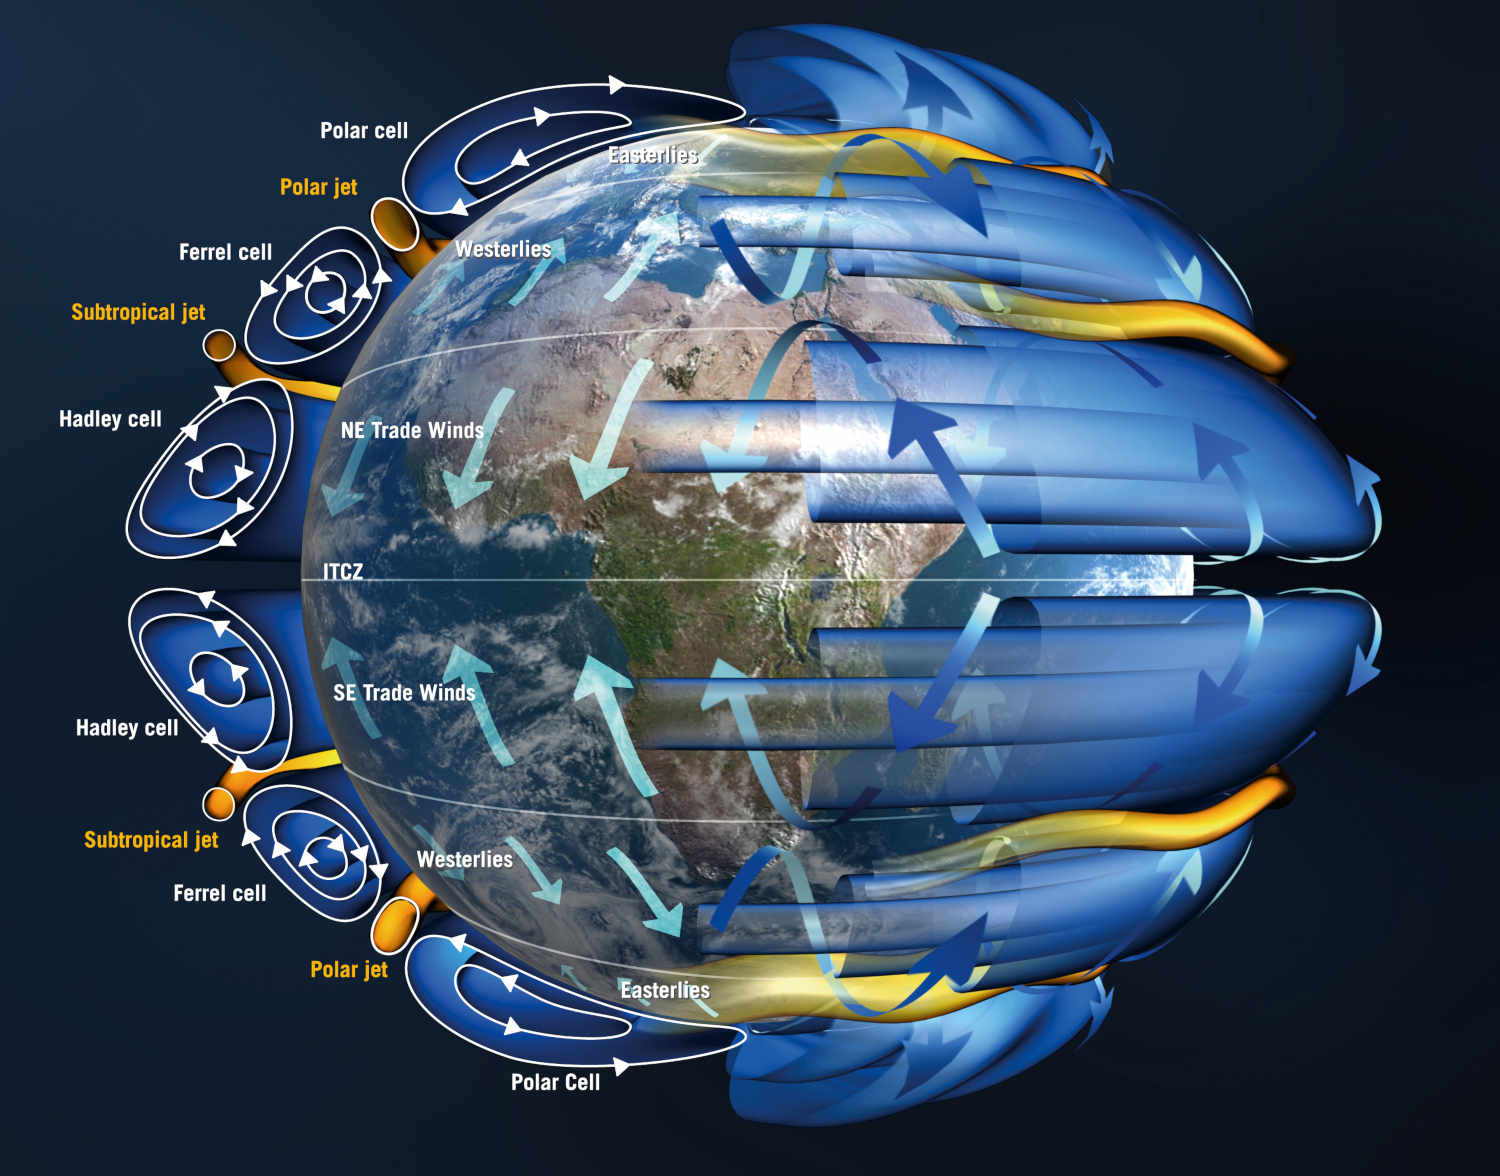
\includegraphics[width=0.8\textwidth]{img/Earth_winds.jpg}
	\caption[Earth winds circulation]{A model of Earth's atmosphere air circulation, transporting heat
	from equatorial regions to poles and returning cooled air to the tropics.
	The circulation in each hemisphere consists of three cells, creating two
	important jets in each hemisphere. Credits: ESA/AOES Medialab \cite{earth_winds}}
	\label{fig:earth_winds}
\end{figure}


Something that would help improving the weather predictions is to better know
the winds profile in every layer of the atmosphere, globally, and with much better
time resolution. This study has been performed in the past by using flying probes
as high altitude balloons, or other unmanned flying devices which were able to
measure the winds speed but in a local area, not in every moment, nor every altitude.\\

The mission ADM-Aeolus is intended to provide this global observations of winds,
for every altitude in the atmosphere and with a resolution that will satisfy the
requirements of the World Meteorological Organization (WMO). ADM-Aeolus will
be the first satellite to directly observe the Earth’s wind profiles from space.
\cite{Endemann2004}\\

The Mission was launched this year on 22 of August onboard of a Vega rocket, manufactured
by the Italian company Avio, from the Guiana Space Centre, one of the usual launch
facilities of the European Space Agency located in Kourou, French Guiana. The total
mass of the satellite is 1360kg, which includes 266kg of fuel, and it is orbiting
Earth in a 320km height sun-synchronous orbit, with an inclination of 96.7º and a period
of 90.7 minutes \cite{aeolus_n2yo.com}, with an estimated lifetime of at least
3 years, due to his relative lower orbit altitude.

\section{Payload: ALADIN}

To accomplish the mission objective of studying the winds in Earth atmosphere, the
selected payload is called ALADIN, which stands for \textbf{A}tmospheric \textbf{LA}ser
\textbf{D}oppler \textbf{IN}strument. This instrument is able to measure the
wind speed and direction in every layer of the atmosphere covering all the Earth.\\

The way in this instrument works is by pointing a UV-LASER beam into the atmosphere
and observing the back-scattered light from it, which would suffer Doppler-effect
due to the velocity of air molecules moving withing the atmospheric currents, as
is depicted in \ref{fig:scanning}, employing the DWL (Doppler Wind Lidar) measuremnent
technique, along the LOS (Line-of-Sight).\\

\begin{figure}[h]
	\centering
	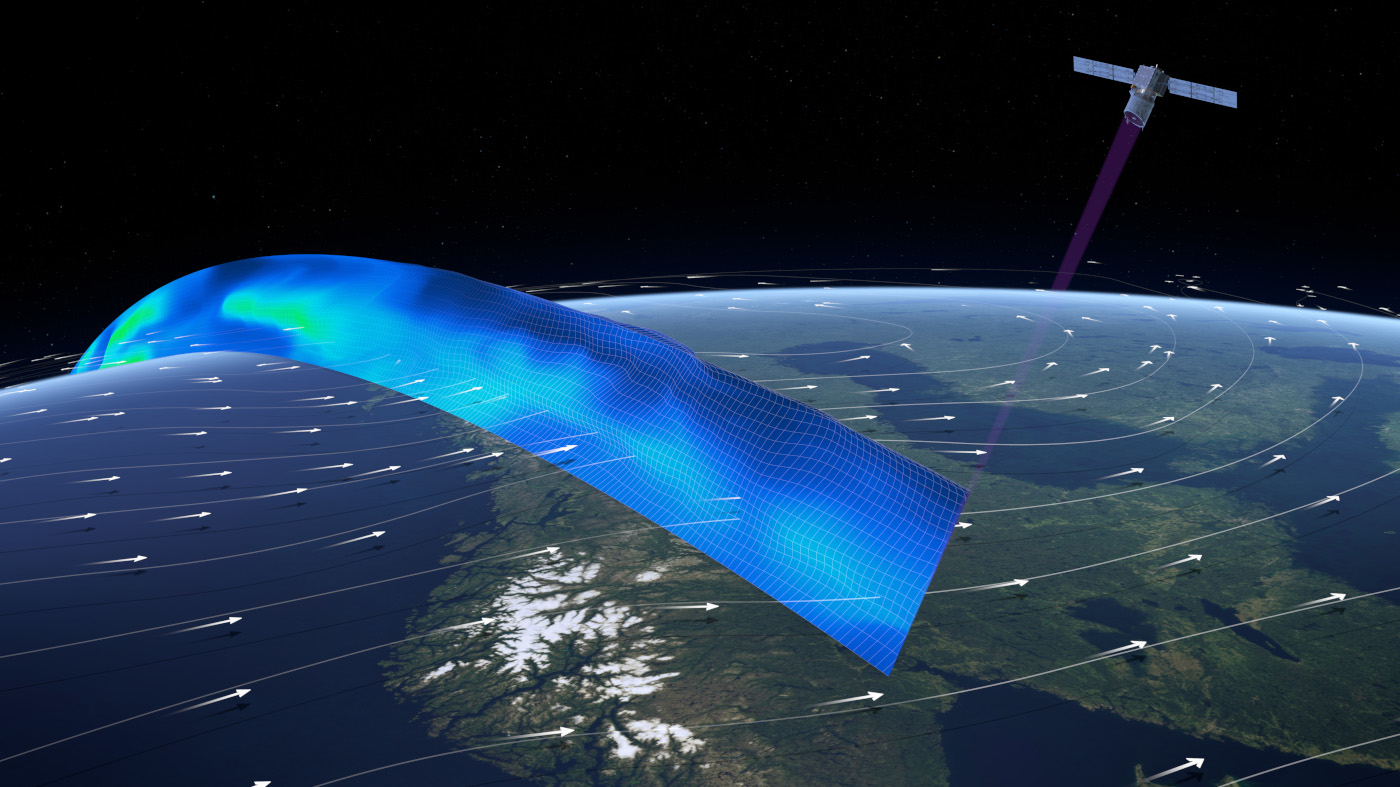
\includegraphics[width=0.9\textwidth]{img/Winds_profile.jpg}
	\caption{Artistic impression of Aeolus scanning Earth winds profiles.
	Credits: ESA/ATG medialab \cite{scanning}}
	\label{fig:scanning}
\end{figure}



The state-of-the-art Aladin instrument incorporates two powerful lasers, a large telescope and very sensitive receivers. The laser generates ultraviolet light that is beamed towards Earth. This light bounces off air molecules and small particles such as dust, ice and droplets of water in the atmosphere. The fraction of light that is scattered back towards the satellite is collected by Aladin’s telescope and measured


% Geometry of the measurements
The wind is observed orthogonal to the satellite ground-track, pointing 35° off nadir, away from the Sun. Observations cover 50 km along the flight direction, and are spaced 200 km apart.
(H)LOS means (horizontal) line of sight

\begin{figure}[h]
	\centering
	%\includegraphics[width=0.5\textwidth]{}
	\caption{A Nicolet Nexus 670 FTIR}
	\label{fig:machinery}
\end{figure}
